\chapter{The eXtensible Markup Language}\label{chap:XML}

Statisticians often need to use different software tools in their data
analysis, and by far and away the most common solution to sharing data
between applications has been to exchange data via ASCII or text
files.  One application will write out its view of some data; the
other application will then read this file and construct its internal
version of this dataset and go about its business. If we want to make
the results of computations in this application available to the
original application or any other, we write the results to another
ASCII file and they are there to be picked up by any other
application.  We don't reserve this style of communication for dynamic
interaction between two applications running simultaneously.  We
exchange datasets in the same way, using agreed upon formats such as
white-space delimited or comma-separated data files.  Since most of
the datasets over the years are rectangular tables or arrays, the
ASCII format is relatively natural.  Each line corresponds to a
record, and each element within a line corresponds to a variable and
is the value for that variable.

The benefits of using tabular ASCII files are easy to see. 
\begin{itemize}
\item We can edit them in simple text editors.  
\item There is a natural connection between the visual layout in the 
  file and the way we think about the dataset when computing on it.  
\item It is quite simple to both write and read data in this format.  
\end{itemize}

But what happens as data become more complex? 
How do we represent \textit{missing values} in our data?  A common
approach is to choose a number that is not in any of our datasets and
to have our software treat such a value in a special way. And so we
see datasets with numbers like `999'.  Of course, the software cannot
be used to read datasets that actually have `999' as an actual value
since it will mark these as missing.  

Another problem arises if we have \textit{repeated measurements} within
records and there are a different number of measurements for each
record.  The data are no longer rectangular and we will have to modify
our software to be able to read and write these files.  Not only that,
how will we tell the software that there are 6 consecutive values for
this record that are to be collected together into a single array, but
for the next record there are only 3? In other words, how do we
separate the different values within a record and associate them with
a given variable.  In the simple table version, each variable in each
record had only a single value. If we have an arbitrary number of
values per variable, a simple way to indicate this in the file is to
put in another variable that tells the software how many values to
expect.  Suddenly, the simplicity of the tabular ASCII file is
disappearing and the software in all the different applications has to
be changed.

Repeated measurements are a simple example of a general problem. Even
within the context of a rectangular array, what if some of the
\textit{entries are objects} rather than simple values?  The least we
should be able to do with good data analysis software is to write out
a dataset and read it back in without losing information. This is
often called \textit{round-tripping}.  If we want to be able to read
these objects, just as for the repeated measurements, we have to be
able to identify that the next $k$ values go to make up the object.
So, again, we are seeing that we have
to add meta-information to the dataset so that our software
can be certain to read it back unambiguously.


In the past, people have distributed a dataset as a collection of
files.  One file contains the actual values and the others contain
information such as the variable names, descriptions of the variables,
information about the origins of the data and how they were collected,
and so on. These additional files are sometimes called the \textit{codebook}.
XGobi, an interactive graphical visualization system, used
a format that consisted of several files to represent the data
(records and variables), variable names, the color of the records, the
glyph for the record, and so on.  One of the major problems with these
multiple file approaches is that it is very easy to edit one file and
forget to update the others. For example, if we remove a record in
the dataset and not in the color specification, the two files no longer
match. At best, we would get an error message about this. Alternatively,
we just get the wrong values for the different records.  Essentially,
having the data in different files reduces the advantage of being able
to edit it in a natural fashion. The visual similarity of the data and
the conceptual model is no longer there.

Not only does the multiple-file approach make editing harder, but it
also makes it harder to distribute.  Nowadays we use HTTP or FTP from
within applications to download files. There syntax for specifying a
collection of files is less natural than giving a single URL.  And
this becomes an issue as we combine datasets together. 

We have focussed on rectangular data arrays since these are probably
the most common form of data that statisticians experience.  Many of
the same problems arise with other formats, and indeed can be worse.
A popular format for name-value pairs is the properties file format 
given either as
\begin{verbatim}
name: value
\end{verbatim}
or
\begin{verbatim}
name=value
\end{verbatim}
With this format, one has to be careful about how white space at the beginning and end
of the value is handled.  And long values that extend onto second and
third lines can be tricky.  Obviously this format is limited to
specific types of data. Like many other formats, it is hard to extend
it to include different types of information.  Again, if we want to do
something as easy as combine multiple sets of name-value pairs, there
is no easy way to separate the sets within the file.

There is a theme inherent in this list of problems associated with
representing ASCII data in simple files.  The basic impediment is that
there is no way to add meta-information to the data.  Ideally, we
would like to be able to include information such as what the missing
value identifier is; identify objects as a collection of (potentially
named) values; include multiple separate but related datasets in a
single file.  We would like the software to be able to read the
meta-information if it is there, and yet not require it to be there
and ignore it if the software doesn't understand it.  The ability to
add meta-information to representations of data would make us more
expressive.  We could differentiate between a real number that has an
integer value and an integer, i.e. the different between $1$ and $1.0$
that often gets lost when software reads ASCII data.  We could refer
to one piece of the data in another part of the data, i.e.
cross-reference the elements, to indicate that if one piece is
updated, the other pieces should reflect this.  Without
meta-information or markup for ASCII data, we are quite limited in
what we can express.

The general markup language, XML -- the eXtensible Markup Language,
allows us to mark up ASCII data with meta-information. 
Just being able to add meta-information via markup allows us to solve
several of the problems mentioned above. 
But we have two other issues to face when looking for a
markup mechanism. Firstly, if we are the only people using it, aren't
we going to restrict our ability to exchange data with other
communities? Since this exchange is becoming increasingly important,
that would be a very bad thing. But again, we are fortunate because
XML is quickly emerging as an extremely popular and widespread general
data format. It is used to represent genetic information, geographical
maps, output from databases, protocol for remote procedure calls
(RPC), authoring technical articles and books, and so on.  Word
processors, spreadsheets, and relational databases now provide options 
to save their contents as XML.

XML's popularity answers the second question that we should ask when
considering using XML to represent data: What is the cost of switching
to XML?  A new format requires us to
rewrite software. This involves retesting our software, etc. which is
a very time consuming task. So if we don't get any tools to help us
write this new software, the cost of switching to XML may well be
excessive. And again, the good news is that since all these other
communities are actively using XML, they are also providing extensive
collections of tools for working with XML. And we can incorporate
those into our environments and get the benefits of XML relatively
transparently.

So what are the drawbacks to XML?
It does solve all of the problems we have identified in the
previous paragraphs. But, like all pieces of software, it is not a
silver bullet that solves all problems and introduces no new ones.
Rather it gives us more options (since we can always use non-marked up
data, even as parts within XML documents), and is a step in our
evolution.  It raises higher-level problems which we will then have to
try to solve while people use XML.  One of the strengths of XML is
that it is structured to make it easy for a computer to read.
However, it leads to very verbose content and it is quite hard for us
humans to read. And that means it is hard to edit
directly. And so we lose the simplicity afforded by raw ASCII data,
which means we need tools that allow us to visualize and manipulate XML content
to create inputs. Or in other words, we need software that reads and
writes the XML and insulates us from the details.  As we will see,
this is not a simple problem in general because XML is itself
extremely general. However, each community will gradually develop
tools for viewing its own types of data and hopefully these will be
shared when possible. Even now, some general tools for editing XML are
emerging and can be customized to our needs.


Now that we have motivated the value of XML, we will go into a little
more detail. We will first give a more precise description of XML and
its parts. Next, we will discuss the \SPackage{XML} package for R
which allow us to both read and write XML directly from within the an
R session.  We will illustrate this package by looking at some real
examples of XML for reading and writing data from other applications.



\section{What is XML?}
The eXtensible Markup Language provides a standard for the semantic 
management of data.  
It is a formal meta-language facility for defining a markup language.
The basic unit in an XML file is an entity
or chunk that contains content and markup.
The content is the actual information such as 6. 
The markup describes the content, in this case the
markup is the name \XMLTag{CYL} for the cylinders
variable in the dataset
(see the example in Section~\ref{sec:XMLSAS}).
More generally, markup consists of tags, attributes, comments,
and processing instructions for the content.
The tag marks the beginning and end of a piece of content. 
That is, content must be surrounded by a start tag 
and a corresponding end tag.

A tag has a name and possibly other pieces of information
describing the element's content.
In a start tag, the name and any additional information are surrounded 
by the \lt and \gt characters. 
Similarly, an end tag consists of the tag name (it must match
the tag name in the start tag) surrounded by \lt/ and \gt. 
For example, the following XML entity
\begin{verbatim}
<CYL> 6 </CYL>
\end{verbatim}
is a \XMLTag{CYL} element with content 6.
It is possible to have empty tags, i.e. tags
with no content,
\begin{verbatim}
<CYL></CYL>
\end{verbatim}
In this case the start and end tags can be combined 
into one tag as follows, \verb+<CYL/>+.

Attributes provide additional information about the content. 
For example, the \XMLTag{dim} tag below has a \XMLAttribute{size} 
attribute which has a value of 2. (See Section~\ref{sec:StatDataML}
for the related example).
\begin{verbatim}
<dim size="2">
\end{verbatim}
Attributes are specified via name-value pairs.
The syntax rules are provided below.


\subsection{XML syntax}

For XML to be \textit{well-formed} it must obey the
following syntax rules.

\begin{itemize}
\item XML is case sensitive so start and end
tag names must match exactly. For example, the following
start and end tags have a mismatch in case and so are not well-formed,
\begin{verbatim}
<CARS>
</Cars>
\end{verbatim}
The end-tag name needs to have all capital letters, i.e. \verb+</CARS>+, 
in order for it to match the start tag.
\item No spaces are allowed between the \lt and the tag name.
\item Tag names must begin with an alpha character, and contain
only alphanumeric characters.
%DEB - what are other restrictions on tag names?
\item  An element must have an open and closing tag unless it is empty.
\item  An empty element that does not have a closing tag must be of the 
form $\&lt; \ldots \&gt;$. For example, \verb+<nan/>+.
\item Tags must nest properly. That is, when one element contains 
another element then the start and end tags of the inner element must 
be between the start and end tags of the parent element.
For example,
\begin{verbatim}
<CARS>
   <CYL> 6 </CYL>
</CARS>
\end{verbatim}
Here the \XMLTag{CYL} tag is nested within the \XMLTag{CARS} tag.
Note the use of indentation makes it easier to see the nesting.

\item All attribute values must appear in quotes in a \verb+name = "value"+
format.
\begin{verbatim}
<dim size="2"/>
\end{verbatim}
This example shows an empty tag with a \XMLAttribute{size} attribute
of ``2''.
\item Isolated markup characters are not allowed in text. 
However, they may be specified via entity references. 
For example, the \lt is specified by the entity reference 
\verb+&lt;+
and the \gt symbol is 
\verb+&gt;+.
\end{itemize}

In addition to element tags, XML has markup for comments, which is
information not shown to the user; processing instructions, which is
similar to code meant for the processor; and character data that is
not to be processed but simply passed straight through to the user.
Comments must appear between \verb+<!--+ and
\verb+-->+. For example, 
\begin{verbatim}
<!-- This is a comment which is so long 
that it apears on three lines of the document
before it ends with -- followed by >. -->
\end{verbatim} 
It is possible to include in a document character
data that is not processed and so the $>$ is ignored.  The character
data must appear between \verb+<![CDATA[+ and
\verb+] ]>+.  
\begin{verbatim}
 <![CDATA[ 
  This is character data that can have any special character 
  in it such as < or > or & and not have to worry about it 
  being interpreted as a special character by the processor.  
]] > 
\end{verbatim} 
Finally, processing instructions must appear between
\verb+<?+ and \verb+?>+.  For example, an XML
document must start with the processing instruction that identifies it
as an xml document and provides the XML version number as an
attribute, \verb+<?xml version = "1.0" ?>+

\subsection{Valid XML}
The rules provided in the previous section are just syntax rules
for insuring that an XML document is well-formed. But we typically want to
have documents that are more than well-formed; we want to include application specific 
structure in the markup. 
For example, with geographic data we may want tags for locations, 
$x$ and $y$ coordinates, city names, etc.  
Tags for these entities are specified through
a set of schema or through Document Type Definitions (DTD for short).
With schema we can: provide the name of a valid element; limit the content
of an element to character data, specific other elements, or to be empty;
and specify the attributes that are required or allowed in the tag.

Well-formed XML obeys XML syntax rules described in the previous section, 
but \textit{valid} XML, in addition to being well-formed, 
obeys a specified schema or DTD.  These may appear within the document
itself or be provided via reference. 
\begin{verbatim}
<!DOCTYPE dataset SYSTEM "../DataSetByRecord.dtd">
\end{verbatim}
Here we specify a DTD to use via a document type declaration.
The \XMLTag{dataset} gives the root element name that the DTD
will be applied to in the verification process.

Occassionally we will generate XML documents that mix content from two
or or more schema.  This flexibility is one of the strengths of XML.
However, it is possible of course that two schema will use the same
element name to mean different things.  And certainly, it is probable
that these two different versions of the apparently same element will
not be valid in the same locations.  To avoid this conflict, we need a
mechanism to be able to differentiate between the two elements and
identify each occurrence with the associated schema or usage.  XML
namespaces provide the mechanism for this.

To make things concrete, consider the case where we are including code
in a document via a \XMLTag{code} element.  We may have code in
different languages such as R and C.  We will want to differentiate
between these two.  We do this by defining unique identifiers for each
namespace in the form of a URI.  We also associate a shorter nickname
with each namespace which we can use as a prefix to elements.  This
prefix tells the XML parser which version of the element was intended
and allows us to use elements in different contexts with full
validation and meaning.

We declare each namespace URI and prefix pair as attributes within an
XML element.  This can be done anywhere in the document so that each
sub-node that uses the namespace can inherit it from parent nodes.

For example, the \XMLTag{object} element below lists three
name space prefixes -- \XMLName{r}, \XMLName{c}, and \XMLName{bioc} -- and
the URI's with which they are associated
\begin{verbatim}
<object xmlns:r="http://www.r-project.org" 
        xmlns:c="http://www.c.org" 
        xmlns:bioc="http://www.bioconductor.org" 
        type="R-pop-environment" hidden="true">
\end{verbatim}
We specify which name space a tag uses within the \XMLTag{object}
element
using the form \verb+prefix:element+, e.g.
\begin{verbatim}
<r:code>
x = rep(23, 2)
</r:code>
<c:code>
for(i = 0; i < n; i++)
  *p++ = *q++;
</c:code>
\end{verbatim}

A parser has the job of reading the XML, checking it for errors, and
passing it on to the intended application.  If no DTD or schema is
provided, the parser simply checks that the XML is well-formed.  If it
is provided then the parser also determines whether the XML is valid,
i.e. that the tags, attributes, and content meet the specifications
found in the schema, before passing it on to the application.  Models for
parsing XML are described in greater detail in sections~\ref{}.

\subsection{XHTML}
Some readers will have thought of HTML when we mentioned markup
and meta-information. 
After all, what is the difference between HTML and XML?
We can add meta information to HTML documents using the \HTMLTag{META} tag, 
but this is not exactly what we mean by meta-information.  
A little thought and familiarity with HTML will quickly bring us to problems. 
HTML has a fixed set of markup elements, e.g. \HTMLTag{H1}, \HTMLTag{H2}, 
\HTMLTag{a}, \HTMLTag{img}, \HTMLTag{B}, and so on.  It doesn't even have a
\HTMLTag{NUMBER} or \HTMLTag{REAL} markup for representing real
numbers. 

An important role of XML is to
separate out information (content) from the structure and format.
The markup provides the structure of the content, and the
the format determines how the content is to be rendered for
viewing by the user. 
As a simple example, an array of numbers that corresponds to the
miles per gallon of various makes of cars may be provided
via XML as follows:
\begin{verbatim}
<array name="MPG" size="7" type="numeric">
  <e>21.0</e> <e>21.0</e> <e>22.8</e> <e>21.4</e>
  <e>18.7</e> <e>18.1</e> <e>14.3</e>
</array>
\end{verbatim}
The content consists of the set of values 
21.0, 21.0, 22.8, 21.4, 18.7, 18.1, and 14.3. 
The structure provided via the markup tells us that the content 
forms an array of numbers of length 7, and the array is named MPG.

HTML does not make the same division between content, structure, and format. 
Many tags describe how to format content, but provide no information about the
type of content.
For example, the HTML tags \HTMLTag{B} for bold face, \HTMLTag{br} 
for line break, and \HTMLTag{hr} for horizontal rule are all
instructions for the visual rendering of content.  

HTML has been extended to XHTML by requiring all tags to be lower case, 
all elements to be properly closed with end tags, and attribute values
to appear between quotes. 
Although these rules mean that we can require XHTML documents to be well-formed and 
valid, XHTML is not up to the job of describing 
complex structures such as factors, data frames, S objects, and so on.
Clearly XHTML is lacking in this regard. 
With XML we can define much richer application-specific markup. 


\section{XML examples}
Data exchange between different software tools typically poses
a problem because different applications use their own, 
proprietary, undocumented formats for data storage. 
The use of a well-defined, common exchange format can help solve 
this problem.
We explore here two proposals for XML-based data exchange formats.
The first is supported by SAS, and the second by R, Matlab, and Octave.

\subsection{SAS}\label{sec:XMLSAS}
The SAS XML library allows you to export an XML document from a SAS 
dataset and to import an XML document into a SAS dataset. 
The XML document below gives an example of XML
data that can be read into SAS.

\begin{verbatim}
<?xml version="1.0"?>
<LIBRARY>  
   <CARS> 
         <ID> Mazda RX4 </ID>
         <MPG> 21.0 </MPG>
         <CYL> 6 </CYL>
         <HP> 110 </HP>
         <AM> 1 </AM>
   </CARS>
   <CARS>  
         <ID> Datsun 710 </ID>
         <MPG> 22.8 </MPG>
         <CYL> 4 </CYL>
         <HP> 93 </HP>
         <AM> 1 </AM>
   </CARS>
   <CARS> 
         <ID> Valiant </ID>
         <MPG> 18.1 </MPG>
         <CYL> 6 </CYL>
         <HP> 105 </HP>
         <AM> 0 </AM>
   </CARS>
</LIBRARY>
\end{verbatim}

The root element in the XML document is denoted by the \XMLTag{LIBRARY} tag.
The tag name for the second-level element represents the
SAS dataset name,
in this case \SASName{CARS}.
Each \XMLTag{CARS} element translates into a record in the SAS dataset.  
We see from the figure that this dataset has 3 records,
one for each of the 3 occurrences of the \XMLTag{CARS} elements.

The variables in the dataset correspond to the 
elements nested within the CARS element. 
The tag names for these elements translate into the variable names. 
That is, ID, MPG, HP, and AM, are the names for 
the variables pertaining to the identification,
miles per gallon, horse power, and automatic/manual transmission
information for the cars.
The content of these elements gives us the value for the
variables in that record.
The first record has the value ``Mazda RX4'' for ID,
21.0 for MPG, etc., 
the second record has the value ``Datsun 710'' for ID,
22.8 for MPG, etc.

Note that this input format handles only rectangular datasets
and that type information, units, and missing values are not specified.
The XML data are read in to SAS and shown below

\begin{verbatim}
libname test xml 'C:\My Documents\test\cars.xml';
proc print data = test.cars;
run;

ID              MPG       CYL       HP       AM

Mazda RX4       21.0      6         110       1
Datsun 710      22.8      4         93        1
Valiant         18.1      6         105       0               
\end{verbatim}

SAS 9.1.3 provides alternatives via XMLMap to include type information
for variables, handle ragged arrays, and to specify a translation of other 
XML formats into the one provided here (see 
\URL{fttp://support.sas.com}).

\subsection{StatDataML}\label{sec:StatDataML}
Meyer, Leisch, Hothorn, and Hornik, proposes a data exchange format 
for statistical data, called StatDataML. 
The R package \SPackage{StatDataML} provides
an implementation of this data exchange format.

An example of XML that obeys the StatDataML requirements for 
importing data from XML into R, Matlab, Octave appears below. 
The content is the same as that shown in the example in 
Section~\ref{sec:XMLSAS}:

\begin{tabular}{lrrrr}
ID &    MPG &    CYL &  HP &   AM \\
\hline
Mazda RX4  & 21.0 &     6 &     110 &   1\\
Datsun 710 &  22.8 &    4 &     93 &    1\\
Valiant    & 18.1 &     6 &     105 &   0
\end{tabular}

The XML document is much more verbose than the SAS example as it includes more
structure.  For example, the variables are typed.  We specify in the
XML elements \XMLTag{type}, \XMLTag{categorical}, and \XMLTag{level}
that the variable \SName{AM} is categorical with the level 0
indicating automatic and level 1 manual transmission.  The StatDataML
format is general enough to describe complex R objects such as lists
of arbitrary content, which means that it must be more verbose than a
data exchange format that assumes a rectangular array.  The data in
this example have the simple rectangular shape, and so can be stored
in a data frame in R.  The data frame is a special case of the list
which forms a rectangular shape where the columns can be arbitrary
types.  Here, our columns are a mixture of character, numeric and
categorical data types.  If we had relied on the inherent structure of
the data frame in describing the strucutre of the data then the XML
would be made more compact by eliminating the \XMLTag{dimension} and
\XMLTag{dim} tags within each \XMLTag{Array} tag would not be
necessary.

%Deb install the package and check to see if 
% we can get along with out it.

\small{
\begin{verbatim}
<?xml version="1.0"?>
<!DOCTYPE StatDataML PUBLIC "StatDataML.dtd">
<StatDataML xmlns="http://www.ci.tuwein.ac.at/StatDataML">  
  <description>
    <title> Cars </title>
    <comment> A subset of the mtcars data from R </comment>
  </description>

  <dataset>
    <list>
      <dimension>
        <dim size = "5">
          <e>ID</e> <e>MPG</e> <e>CYL</e> <e>HP</e> <e>AM</e>
        </dim>
      </dimension>
      <listdata>
        <array>
          <dimension> <dim size="3"/> </dimension>
          <type> <character/> </type>
          <data>
            <e> Mazda RX4 </e> <e> Datsun 710 </e> <e> Valiant </e>
          </data>
        </array>
        <array>
          <dimension> <dim size="3"/> </dimension>
          <type> <numeric/> </type>
          <data>
            <e> 21.0 </e> <e> 22.8 </e> <e> 18.1 </e>
          </data>
        </array>
        <array>
          <dimension> <dim size="3"/> </dimension>
          <type> <integer/> </type>
          <data>
            <e> 6 </e> <e> 4 </e> <e> 6 </e>
          </data>
        </array>
        <array>
          <dimension> <dim size="3"/> </dimension>
          <type> <numeric/> </type>
          <data>
            <e> 110 </e> <e> 93 </e> <e> 105 </e>
          </data>
        </array>
        <array>
          <dimension> <dim size="3"/> </dimension>
          <type> 
            <categorical mode="unordered">
              <label code="0">Automatic</label> 
              <label code="1">Manual</label> 
            </categorical> 
          </type>
          <data>
            <e> 1 </e> <e> 1 </e> <e> 0 </e>
          </data>
        </array>
      </listdata>
    </list>
  </dataset>

</StatDataML>
\end{verbatim}
}

We provide a brief description of the elements of this StatDataML
document.

\begin{itemize}
\item The name of the document containing the DTD is provided in
the \XMLTag{DOCUMENTTYPE} element.
\item The root element of the document is \XMLTag{StatDataML}.
It contains two elements, the 
\XMLTag{description} element and the \XMLTag{dataset} element.
\item The \XMLTag{description} element contains information pertaining
to the source of the data. 
\item The \XMLTag{dataset} element contains the data along with
all the markup describing it.
\item The data may be a simple array or a list. In our case, we have
a list object and so use the \XMLTag{list} element. Notice that
it contains 5 \XMLTag{array} elements, one for each column of the 
data frame.
\item The first \XMLTag{dimension} tag provides information about
the number and names of arrays in the dataframe. We see that there
are 5 columns, and their names are provided via the \XMLTag{e} tag.
\item The other \XMLTag{dimension} tags appear inside the 
\XMLTag{array} elements and provide information about the length
of the array. 
\item Information about the data type is provided in the array
element via the \XMLTag{type} entity.
Notice that this tag has no content, i.e. it is empty in all cases
because the data type is provided via a \XMLTag{numeric},
\XMLTag{character}, or \XMLTag{categorical} tag.
\item Finally, the \XMLTag{data} entity provides the values of the
variables. Rather than prividing this information one record at a
time, it is provided one variable at a time. This approach is 
more condusive to the list data structure.
\end{itemize}

\section{The XML document as a tree}
The indentation used in the examples in Sections~\ref{sec:XMLSAS} 
and~\ref{sec:STatDataML} are suggestive of a tree structure.
Each tag can be tought of as a node in the tree, and branches
eminate from the node if the entity corresponding to the tag
contains other tags or content.
The conceptual model of the document as a tree can be very
helpful when processing or navigating a document.
In fact one of the two standards for parsing an XML document, 
is the Document Object Model, or DOM for short, which
reads the XML content and returns a data structure that
represents the document as a tree. The DOM parser is described 
in detail in Section~\ref{sec:DOMParser}. 

\begin{figure}
{\footnotesize{
\begin{verbatim}
LIBRARY   
|
|--CARS 
|  |--ID
|  |  |-- Text
|  |      |--Mazda RX4 
|  |--MPG
|  |  |-- Text
|  |      |--21.0
|  |--CYL
|  |  |-- Text
|  |      |--6
|  |--HP
|  |  |-- Text
|  |      |--110
|  |--AM
|     |-- Text
|         |--1
|
|--CARS 
|  |--ID
|  |  |-- Text
|  |      |--Datsun 710
|  |--MPG
|  |  |-- Text
|  |      |--22.8
|  |--CYL
|  |  |-- Text
|  |      |--4
|  |--HP
|  |  |-- Text
|  |      |--93
|  |--AM
|     |-- Text
|         |--1
|
|--CARS 
   |--ID
   |  |-- Text
   |      |--Valiant 
   |--MPG
   |  |-- Text
   |      |--18.1
   |--CYL
   |  |-- Text
   |      |--6
   |--HP
   |  |-- Text
   |      |--105
   |--AM
      |-- Text
          |--0
\end{verbatim}
}}
\caption{A tree depicting the SAS-XML document found in 
Section~\ref{sec:XMLSAS}}
\label{fig:SASXMLtree}
\end{figure}

Figure~\ref{fig:SASXMLtree}
represents the XML document from the SAS example
in Section~\ref{sec:XMLSAS} as a tree.
The \textit{root} of the tree is the document node,
which in this case is the LIBRARY node.
There is only one root node per document, and 
it is the top-most node, i.e. the \textit{parent} of all other nodes. 
Notice that the LIBRARY node has four children,
each one a CARS node, one for each record in the dataset.
Also note that the character content of an entity is 
always placed under a Text node. 
The terminal branches of the tree are known as \textit{leaf nodes}.  
By design, the character content of an entity will always fall in a leaf node,
as the child of a Text node. 
Each node in the tree has information associated with it:
its name (i.e. the tag name or ``Text''), attributes if it has any, 
and  a list of its children.
In the following sections, we will see how this conceptual
model will help us manipulate the contents of a document to
create S objects, etc.


\subsection{Reading XML as a tree}
There are two styles of XML parsers: DOM and SAX parsers.  
DOM stands for Document Object Model and DOM
parsers read the XML content and return a data structure that
represents an XML tree as shown above.  
The parser sweeps over the entire document and returns an appropriate 
representation of a tree in the programming language.
The tree contains each of the XML elements and its attributes, and 
clearly represents the relationships between them. 
Essentially a DOM parser returns a copy of the XML document but
in a form that makes is easier to operate on the document 
and convert its contents as you wish. As a tree, you can perform multiple
passes over the tree and perform arbitrary transformations.
We give examples of this in the next section.

SAX stands for Simple API for XML. It is qute
different from DOM in that all it does is call different
application-specific handlers as it encounters different parts of the
XML content.  The SAX parser doesn't try to build the XML tree.
Instead, it passes small pieces of information about the XML content
to the event handlers and they are responsible for determining how to put
these pieces together and convert the XML document into data that is
meaningful to the application.  The SAX parser is very low-level.  It
calls the handlers when a new XML element is opened and again when
it is closed. It passes information to the handlers when it sees an
XML comment or a processing instruction.  It is really quite basic and
almost all of the hard work is done in the application-specific handlers.  
However, where SAX parsers become important is when the XML tree 
that a DOM parser would create is very large.  
Rather than reading the entire XML document and processing it to create a 
large ``tree'' object, the SAX parser allows us to incrementally create the
data object without holding the XML tree in memory.  Since we get to
see very small parts of it in the handlers, they need only
remember enough to make sense of subsequent pieces.  And typically
these handlers work very locally and so keep a very small amount of
information across calls.  So SAX parsers are more efficient when
large XML documents are being read, but require more thought in
programming and are more complex to use.

The \SPackage{XML} package for the S language provides both a DOM and
SAX parser via the \SFunction{xmlParse} and
\SFunction{xmlEventParse} functions respectively.  These have an
S-style to them, but if you use them in the default manner, they are
for the most part the same as the general DOM and SAX parsers.
In addition to DOM and SAX based parsers, the \SPackage{XML} package
provides a hybrid parsing model.  DOM reads the entire tree using the
basic mapping for XML elements to S objects. SAX requires callbacks at
a very detailed level, i.e. start and end of XML elements, rather than
at the XML element or object level.  The hybrid style allows us to
use the DOM style of parser but to have handlers or callbacks that work
on entire XML elements.  This allows us not to store the entire tree,
but to deal with it in chunks that are natural to process.  We don't
have to deal with all ``events'' or chunks as we do in the SAX model.
Instead, we can tell the parser the names of the XML chunks we want to
deal with and it will use the default handlers to build the tree for
the chunks we ``ignore''.  This combines efficiency with ease of
programming and allows us also to employ either of the regular models


\subsection{Input Sources}
In most cases, the XML content that we want to parse will be in a
local file.  In such cases, we just pass the name of this file to
\SFunction{xmlParse} or \SFunction{xmlEventParse} via the
\SArg{file} argument.  In other contexts, we will have the XML
document as an S string. This can occur when we either create the XML
internally within S and keep it in memory rather than writing it to a
file.  Also, we may read a file and extract only a portion of it to
get the XML content of interest.  Rather than write this string to a
temporary file and passing that to the XML parser, we can pass the
string directly to the parser and have it work on that.

Since we often use XML to exchange data with different, potentially
remote, applications, it is convenient to be able to put the XML
source on a Web site. Rather than having the user explicitly download
the file, it is desirable to allow him to pass the URL to the parser and
have it parse the content as it reads the file directly from the
server. The libxml parser which we use in the \SPackage{XML} package
does this for FTP and HTTP URIs.  It transparently recognizes URIs and
talks to the server. Rather than using a two step approach of
downloading the file and then parsing it, the XML parser streams the
data incrementally from the server and processes it on the fly.

We have seen that XML is very verbose. This means that it consumes a
lot of disk space when stored or bandwith when sent across a nework.
But if we look at an XML file, we will also see that there are a lot
of repeated patterns.  This tends to make XML content highly
responsive to compression.  Typically ratios of original to compressed
form range between $10$ and $30$\% This wouldn't be exceedingly useful
if we had to manually uncompress the file before handing it to the XML
parser.  However, the libxml parser knows how to read compressed files
and transparently parses the XML directly from that.  While this is
slightly slower than reading the uncompressed file (since it has to
also uncompress the data as it sees it as well as do the usual
parsing), it again provides us with options that allow us to implement
context-specific solutions.

So the XML parser allows us to read from local files, XML strings,
URIs and compressed files.  Unfortunately, it does not support reading
from compressed remote URIs. In such cases, within R you can first
download the URI to a local file using \SFunction{download.file} and
then parse it as is.

\section{The DOM Parser}
The \SFunction{xmlParse} function provides the DOM parsing
functionality in the \SPackage{XML} package.  The basic way to use
this function is to pass it the name of an XML file or URI, or simply a string
containing the XML content.  This is the only required argument for
the function. The others control how the parsing is done and the
different elements handled. 
Let's focus on a simple example. Suppose we have an XML representation of 
a matrix given by the following:
\begin{verbatim}
<matrix nrow="3" ncol="2">
 <columnNames><string>X</string><string>Y</string></columnNames>
 <row id="a"><real>1</real><real>2.0</real></row>
 <row id="b"><real>10</real><real>1.2</real></row>
 <row id="c"><real>20</real><NA/></row>
</matrix>
\end{verbatim}\label{eg:XML:matrix}
We can have this as a file, say \file{matrix.xml}
or directly as a string (say, \SVariable{x}) in S.
To parse this, we use 
\begin{verbatim}
x = xmlParse("matrix.xml")
\end{verbatim}
The important bit for our purposes is given in the \SField{children}
element of the resulting list returned from \SFunction{xmlParse}.  We
can access the root node (and so its children) using the
\SFunction{xmlRoot} function.
\begin{verbatim}
 xtree = xmlRoot(xmlParse("matrix.xml"))
\end{verbatim}

Printing this XML tree should produce something very close to the
original XML input, just printed in a slightly different and more
verbose manner. For example, the \XMLTag{NA} is displayed with a start
and end tag.  Eventhough the tree may look like a simple copy of the
XML input, it is not.  It is a tree made up of nodes (see Figure ...),
where each node can potentially have children nodes, with those nodes
also having children, and so on.  These nodes can be accessed as
elements in a list in R are accessed, i.e. with \verb+[ ]+.

The basic XML node in S is an object of class \SClass{XMLInternalNode}.  We
can access its tag name using \SFunction{xmlName}.  Similarly, we use
\SFunction{xmlAttrs} to get the attributes for the node.
For example, working with the root of the XML tree, \SVariable{xtree},
we get
\begin{verbatim}
xmlName(xtree)
[1] "matrix"
a = xmlAttrs(xtree)
a
nrow ncol 
 "3"  "2" 
a[["nrow"]]
[1] "3"
\end{verbatim}

We can get the list of children in an \SClass{XMLInternalNode} using
\SFunction{xmlChildren}.  This returns a named list of the children.
The names are the XML tag names of the children and the elements are
full \SClass{XMLInternalNode} objects.  The number of children nodes can be
computed using \SFunction{xmlSize}.
We can treat the node as if it were an S list of the children and 
use the familiar
subsetting operations \SFunction{[} and \SFunction{[[} to access the
children.  So, if we wanted to get the \SClass{XMLInternalNode} for the first
row of the matrix, we would ask for the second child using
\SExpression{xtree[[2]]}.  We can also index the children by the XML
tag name. So we can get that same row using
\SExpression{xtree[["row"]]}.  Note that this returns the first
element in the list that matches this name.  The node lists are
slightly unusual in that they allow multiple elements to have the same
name. 


For simplicity, there are XML versions of the \SFunction{apply} and
\SFunction{sapply} functions. These are \SFunction{xmlApply} and
\SFunction{xmlSApply} and each takes an \SClass{XMLInternalNode} as its
primary argument.  They iterate over the node's children nodes,
invoking the given function and returning the list of results.  We can
use this to, for example, find the number of children each of the
second-level nodes has:
\begin{verbatim}
xmlSApply(xtree, xmlSize)
columnNames         row         row         row 
          2           2           2           2 
\end{verbatim}
We can supply an arbitrary function in the \SFunction{xmlApply} that
takes a single argument which is the \SClass{XMLInternalNode} and it can
return any S value.  


As we mentioned earlier, the XML parser by default maps XML elements
within the document to \SClass{XMLInternalNode} objects in R.  But there are
different possible types of XML elements within a document. There are
CDATA/literal text nodes, simple text nodes which have only text
rather than sub-nodes, processing instruction nodes and comment nodes.
As the XML parser encounters each node, it knows what type of node it
is and it maps it to the corresponding S object.  
For example, let's read the following XML file:
\begin{verbatim}
<top>
<![CDATA[
 Literal text include & and <
]]&gt;
<?S print(1:10)?>
<TextNode>This is a simple text node</TextNode>
<!--This is an example of all the different type
    of XML nodes that we support in the XML package. -->
</top>
\end{verbatim}
We read it using \SFunction{xmlParse} and
get the root node using \SFunction{xmlRoot}.
\begin{verbatim}
v = xmlRoot(xmlParse("nodeTypes.xml"))
xmlSApply(v, class)
$text
[1] "XMLCDataNode" "XMLNode"     

$R
[1] "XMLProcessingInstruction" "XMLNode"                 

$TextNode
[1] "XMLNode"

$text
[1] "XMLComment" "XMLNode"   
\end{verbatim}
We can look at the individual nodes in the usual manner using
\SFunction{[[} and see what they have in them.  Since these are
extensions of the \SClass{XMLInternalNode}, the usual methods apply to these
also.  However, the content of each of these types of nodes is not in
children but in the text they contain.  To access this content, we use
the \SFunction{xmlValue} function.  In each case, this returns the
node-specific content as a string.  For example, to get the content of
the S processing instruction, we use the expression
\SExpression{xmlValue(v[["S"]])} and get back \SOutput{"print(1:10)"}.

Note that in our example, the \XMLTag{TextNode} element is mapped to a
regular \SClass{XMLNode} in S. It is the first (and only) child that
is the \SClass{XMLTextNode} object.  This makes sense since the
\XMLTag{TextNode} element may have attributes, etc.  whereas the text
node won't .
Hopefully looking at the node and its children
will help to emphasize this point.
\begin{verbatim}
v[["TextNode"]]
 <TextNode>
 This is a simple text node
 </TextNode>
xmlSize(v[["TextNode"]])
[1] 1
class(v[["TextNode"]][[1]])
[1] "XMLTextNode" "XMLNode"    
\end{verbatim}
For more complex nodes, such as \SVariable{v} itself, it returns
\SNull rather than raising an error.


Along with the XML tree, \SFunction{xmlParse} returns auxillary
information about the parsed XML.  Essentially there are two parts to
the result: the document and the DTD.  The document is accessed via
the \SField{doc} element of the returned list and it has information
about the source of the XML input and the version of XML.  The
\SField{file} field in the \SField{doc} object gives the name of the
file that was processed containing the XML (or simply
\verb+"&lt;buffer&gt;"+ if the content was given directly as a string).
The \SField{version} field tells us the version of XML used to author
the document.  This is almost always the value $1.0$ and is the value
you will often see at the top of each XML file to identify the file as
being XML
\begin{verbatim}
<?xml version="1.0"?>
\end{verbatim}

Unless you ask it not to, \SFunction{xmlParse} will try to read
the DTD associated with the XML content.  And it returns this
information as the second part of the result returned from
\SFunction{xmlParse} via the \SField{dtd} field.  This includes
both the external and internal DTD, as each is available, and these
can be accessed via the \SField{external} and \SField{internal}
fields.  
If you are not interested in the DTDs, you can avoid processing them
using the \SArg{getDTD} argument.  Giving a value of \SFalse{} for
this means that only the document part of the result is returned.

At this point, we have covered the structure of XML nodes in S.  We
can now turn our attention to processing the tree and customizing the
XML parser.


\section{Walking the DOM Object}
One way to process XML content into data in S is to use
\SFunction{xmlTreeParse} to read the XML into an S tree or DOM.  Then,
we can extract the pieces of it that we want in any order and
construct the appropriate S object.  Let's return to our matrix
example above on page \ref{eg:XML:matrix} and see how we can create
the appropriate S matrix.

We start by generating the XML tree in S.
\begin{verbatim}
d = xmlRoot(xmlParse("matrix.xml"))
\end{verbatim}
There are several different ways we can proceed.  We can create an
empty matrix with the appropriate dimensions and then fill in the
values and the row and column names.  Alternatively, we can collect
the values into a vector and the row and column names also, and then
create the matrix in a single operation.  The code for either approach
is quite similar and we can focus initially on the common aspects.  

To get the row names, we want to extract the \XMLAttribute{id}
attribute from each of the \XMLTag{row} elements.  We can exploit the
fact that we know the \XMLTag{row} elements correspond to nodes $2$,
$3$ and $4$, or more generally $2, \ldots, \hbox{nrow}$.
Alternatively, we can process each node and check that it is
a \XMLTag{row} element by examing its tag name.
If it is, then we extract its \XMLAttribute{id} attribute.
The following use of \SFunction{xmlApply} does the job of collecting
the row identifiers. The first node (\XMLTag{columnNames}) returns
\SNull, and so we need \SFunction{unlist} to get the individual
names.
\begin{verbatim}
unlist(xmlApply(d, function(x) 
                      if(xmlName(x) == "row") 
                         xmlAttrs(x)[["id"]]))
\end{verbatim}
Getting the column names is a little simpler.  We know there is only a
single node named \XMLTag{columnNames} and we can access it directly
as \SExpression{d[["columnNames"]]}.  To get the individual values in
this tag, we need to process its children and use the
\SFunction{xmlValue} function to get the actual string values.
Again, using \SFunction{xmlSApply} does the job in the simple expression:
\begin{verbatim}
 xmlSApply(d[["columnNames"]], xmlValue)
\end{verbatim}

We can get the dimensions of the matrix directly from the \XMLTag{matrix} element's
attributes and converting them to integer values.  This is easily done
as
\begin{verbatim}
 a = xmlAttrs(d)
 r = as.integer(a[["nrow"]])
 c = as.integer(a[["ncol"]])
\end{verbatim}
We might be tempted to convert all the values in the attributes vector
to integers since we know it only contains the \XMLAttribute{nrow} and
\XMLAttribute{ncol} values.  However, if we were to use this code for
processing a different file and there were other attributes such as
the name of the matrix, or the name of the default type of its
elements, converting these values to integers would be a problem.

The last remaining part of the computation is to get the values for
matrix entries.  Again, we can use \SFunction{apply} or
\SFunction{xmlApply} to loop over the \XMLTag{row} nodes.  Within each
row, we mimic how we got the column name strings by using
\SFunction{xmlSApply} and converting the individual \XMLTag{real} and
\XMLTag{NA} nodes.  Rather than processing each node and checking
whether it is a \XMLTag{row} element, we will simply work on the nodes
$2, \ldots, r+1$ since we know these correspond to the rows.
(If we really know that there are only \XMLTag{columnNames}
and \XMLTag{row} nodes and all the \XMLTag{row} nodes are last,
we could also use \SFunction{xmlSize} to determine the number
of nodes and subtract $1$ to get the number of rows.)
\begin{verbatim}
 m <- sapply(d[2:(r+1)], 
             function(x) 
               xmlSApply(x, 
                         function(x) 
                           ifelse(xmlName(x) == "NA", 
                                  NA, 
                                  as.numeric(xmlValue(x[[1]])))))
\end{verbatim}
We must use \SFunction{sapply} on the resulting list of nodes
(\SExpression{d[2:(r+1)]}) since this, of course, is not an
\SClass{XMLNode}.  The function works on the nodes within each row.
Because of the way \SFunction{apply} (and hence \SFunction{xmlSApply})
works, the result is actually a matrix whose columns correspond to the
values in each of the \XMLTag{row} elements in the XML.
So all we need to do is transpose this
and set the row and columnames.

We can put all the steps together and create
a function that does this, given the root XML node.
\begin{verbatim}
xmlMatrix =
function(node)
{
 a <- xmlAttrs(node)
 r <- as.integer(a[["nrow"]])
 m <- sapply(node[2:(r+1)], 
              function(x) 
                xmlSApply(x, function(x) 
                          ifelse(xmlName(x) == "NA", 
                                 NA, 
                                 as.numeric(xmlValue(x[[1]])))))
 m <- t(m)
 dimnames(m) <- list(unlist(xmlApply(node, 
      function(x) {
          if(xmlName(x) == "row") {
            xmlAttrs(x)[["id"]])), 
            xmlSApply(node[["columnNames"]], xmlValue))
 m
}
\end{verbatim}
And we can use this in calls
such as 
\begin{verbatim}
 xmlMatrix(xmlRoot(xmlTreeParse("matrix.xml")))
\end{verbatim}

You should verify that you know how to implement the other approach
in whch we first create the empty matrix and fill in its values.


\section{Customizing the DOM Parser}
Getting the actual values from the \XMLTag{real} and \XMLTag{NA} nodes
within the \XMLTag{row} nodes was a little cumbersome in the matrix
example.  It would be more convenient if we could simply turn these
into numbers as they were being added to the XML tree in S.  In the
particular case of the matrix, it would be even more convenient to
process each \XMLTag{row} element in the XML input and have it hold
its values as a vector.  In other words, it would be useful to have a
processing step that converted the default XML node created by the XML
parser into an S object that is more suitable for the particular
context.

The \SFunction{xmlTreeParse} function allows us to specify
pre-processing hooks via its \SArg{handlers} argument.  This is
expected to be a named list of functions.  If the
\SArg{handlers} argument is specified, the
XML parser consults it each time it attempts to add an XML node to the
S tree.  It looks at the name of the XML element and searches for an
element in the \SArg{handlers} list with this name.  If it finds such
an entry, it calls that function and passes it the S object
representing the XML node.  It takes the return value from this call
and, if it is non-\SNull, it adds that value to the tree.  If it is
\SNull, it drops that node from the tree.  If there is no matching
element in the \SArg{handlers} list, then the parser looks for a
general function in that list for handling the particular type of XML
node and uses that if it exists in the same way as a more specific
function.  The association between node type and function name in the
\SArg{handlers} list is given in table
\ref{tbl:XML:GeneralDOMHandlerNames}.

% Fix the ']] >' here.
\begin{table}[htbp]
  \begin{center}
    \leavevmode
    \begin{tabular}{lll}
Node Type  & Example & function name \\
XML element & \verb+<node>...</node>+ & startElement \\
Text node & Simple text inside node & text \\
Comment node & \verb+<!-- a comment -->+ & comment \\
CDATA node & \verb+<![CDATA[ literal ..]] >+ & cdata \\
processing instruction &  \verb+<?S 1:10?>+ & processingInstruction \\
XML namespace  & \verb+<a xmlns:name="http://www....">+ & namespace \\
entity reference &  \verb+&gt;+ & entity  \\
    \end{tabular}
    \caption{DOM handler names for XML node types}
    \label{tab:GenrealDOMHandlerNames}
  \end{center}
\end{table}


\subsection{Election results from the web} 
The data of interest are presented via a 
\HTMLTag{table} in a web page. 
The \HTMLTag{table} tag names and attributes contain no useful 
information about the data; they just get in the way of finding 
the data.

\begin{figure}
%XX 
\includegraphics[height=.8\textheight,width=.6\textwidth]{AZScreenShot}
\caption{A screen shot of the county election results for Arizona in
the 2004 presidential election, as shown on the USA Today website,
Note all of the advertizing and additional information that will need
to be discarded in the extraction of the numbers of interest.
}
\label{fig:AZScreenShot}
\end{figure}


\begin{figure}
%XX 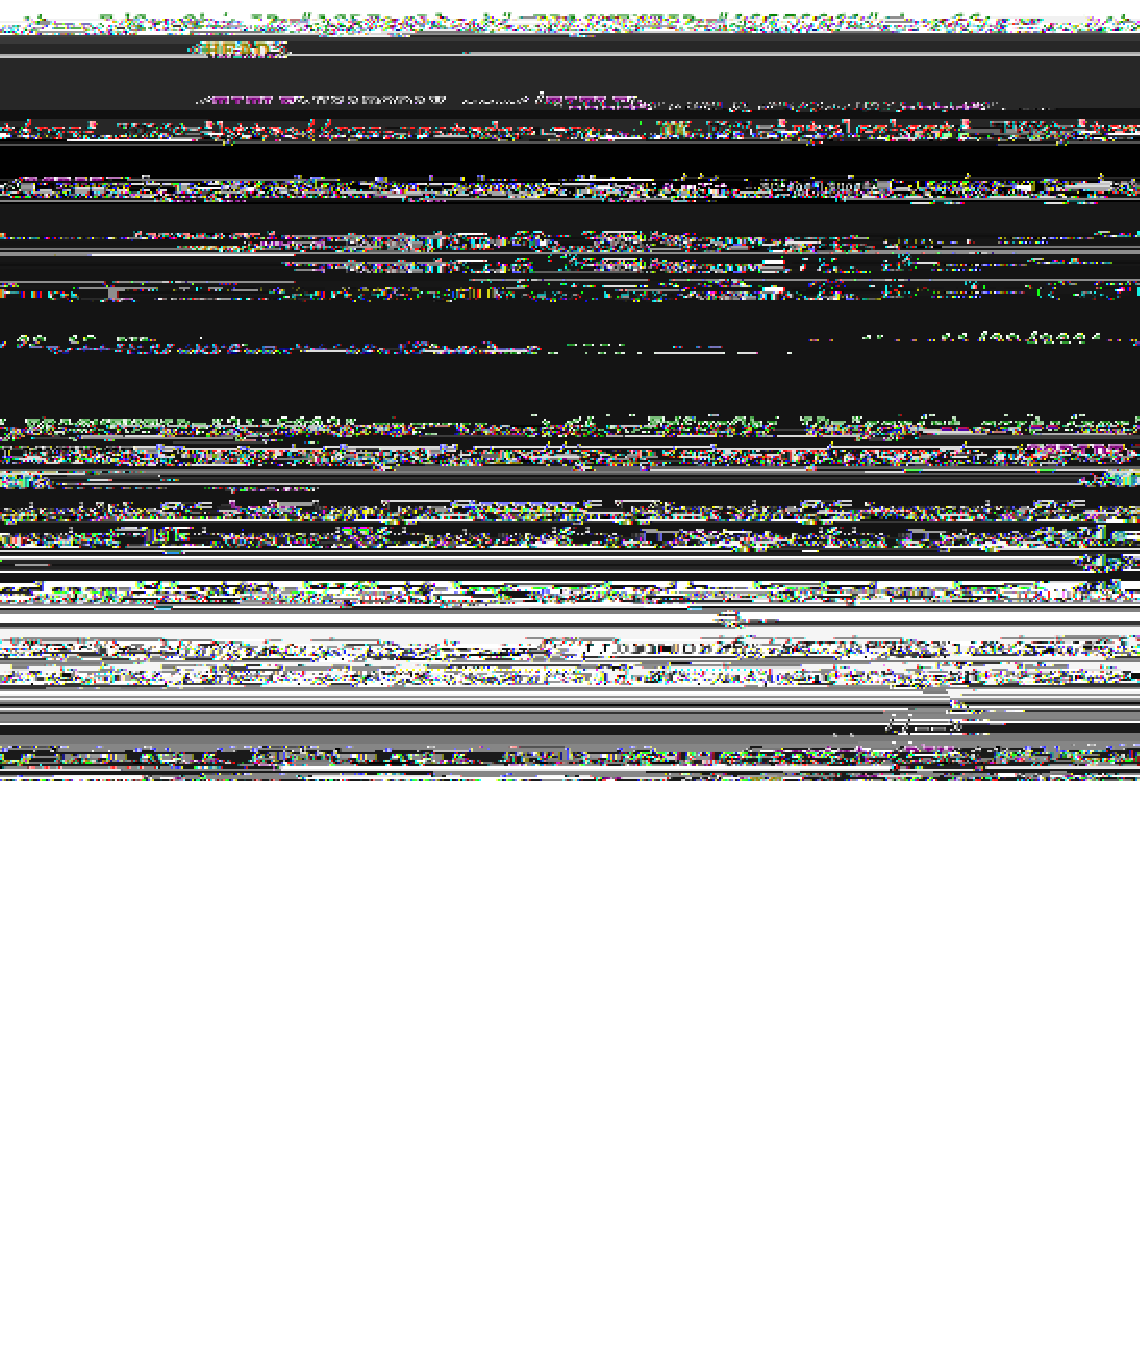
\includegraphics[height=8in,width=5in]{AZSourceScreenShot}
\caption{A screen shot of a portion of the HTML source for the USA Today
web page (shown in Figure xx that presents the
county election results for Arizona in the 2004 presidential election.
}
\label{fig:AZSourceScreenShot}
\end{figure}

Figure~\ref{fig:PAelectionScreenShot} shows a portion of the web page
that contains the table of election results.
We see that the table of interest is embedded in a page with a lot
of extraneous information which we must sort through to find the 
numbers we wish to extract. 
This page is from the USAToday website, where there
is one page for each state; the figure shows us the election results 
from Arizona which can be found at the following URL,
\begin{verbatim}
www.usatoday.com/news/politicselections/vote2004/
  PresidentialByCounty.aspx?oi=P&rti=G&tf=1&Sp=AZ
\end{verbatim}
Notice that the question mark and ampersands in the URL indicate
that the page is dynamically generated from the submission of 
a form with particular parameter values.
In fact, to obtain this page, we selected ``Arizona'' from a 
pull-down menu on a previous USAToday web page.
The Sp argument has the value ``AZ'' to denote that we are 
requesting the data for Arizona.
In Chapter~\ref{chap:electionMaps}, we extract data for all states, 
but for this example we examine only the data for Arizona.  

To get hold of the page, we use the \SFunction{getForm} function 
in the \SPackage{RCurl} package.
\begin{verbatim}
library(RCurl)
usaToday = "http://www.usatoday.com/news/politicselections/
            vote2004/PresidentialByCounty.aspx"
html = getForm(usaToday, oi = "P", rti = "G", tf = "l", sp = "AZ")
\end{verbatim}
The format of the page is identical across states so we can
directly pull the table of interest from the DOM tree and proceed to add
the values of the \HTMLTag{td} tag in a table row (\HTMLTag{tr}) 
to the row in data frame. 
Alternatively, we could use a handler to find the \HTMLTag{table}
nodes and extract data from the table of interest.
To find the table, we run the HTML through the \SFunction{htmlParse}
function in the \RPackage{XML} package and start to walk the tree.
The snippet of HTML source for the Arizona page 
(Figure~\ref{fig:SourceScreenShot})
shows that we have our work cut out for us.
\begin{verbatim}
tree = htmlParse(html, asTree = TRUE, asText = TRUE)
tree = tree[["children"]][["html"]][["body"]]
tree = tree[[1]][[4]][[3]][[3]][[7]][[1]][[6]]
                [[3]][[3]][[1]][[1]]
\end{verbatim}
The table we are after is very deep in the tree.
Rather than rely on the structure of the HTML page in this way,
we can employ a handler function to pull out the correct table
as the parser comes across \HTMLTag{table} tags.
In this case, we do not need to keep the entire
DOM, only the children of the correct \HTMLTag{table} tag interests us.
The \SFunction{tableHandler} function below checks to see if
the first row of a table has the character string,
``Presidential Results - By County'', for its value
as that is the table we are after.
The \SFunction{.value} function returns the table of interest.
Notice that the \SFunction{tableHandler} function assigns
the correct table into \SVariable{countyTable} in its parent environment 
by using the \verb+<<-+ double arrow assignment.
The \SFunction{.value} function also has access to the
\SVariable{countyTable} object in its parent namespace.
A call to \SFunction{.value} returns the current value of
\SVariable{countyTable}.
\small{
\begin{verbatim}
tableHandlers =
function()
{
  countyTable = character(0)
  tableHandler = function(x){
     if (!is.null(xmlValue(x[[1]]))) {
      if (xmlValue(x[[1]]) == "Presidential Results - By County")
             countyTable <<- x
     }
  }

  list(table = tableHandler, .value = function() countyTable)
}

 tree = htmlTreeParse(html, asTree = FALSE, asText = TRUE,
             handlers = tableHandlers())$.value()
\end{verbatim}
}
Once we have that table of interest, we examine the content of the rows.
The first two rows and the last row can be discarded as they
do not contain county information.
The \SFunction{xmlValue} function is very handy in extracting the
data we are after.

\begin{verbatim}
xmlName(tree)
[1] "table"
names(tree)
 [1] "tr" "tr" "tr" "tr" "tr" "tr" "tr" "tr" "tr" "tr" "tr" "tr" "tr" 
[14] "tr" "tr" "tr" "tr" "tr"
tree[[4]]
 <tr>
  <td class="notch_light" width="153">
   <b>
   Cochise
   </b>
  </td>
  <td class="notch_light" align="Right" width="65">
  64
  </td>
  <td class="notch_light" align="Right" width="70">
  64
  </td>
  <td class="notch_light" align="Right" width="60">
  24,828
  </td>
  <td class="notch_light" align="Right" width="60">
  16,219
  </td>
  <td class="notch_light" align="Right" width="60">
  0
  </td>
 </tr>
]
xmlValue(tree[[4]][[1]])
[1] "Cochise"
xmlValue(tree[[4]][[4]])
[1] "24,828"
\end{verbatim}
Notice that the attrivbutes on the \HTMLTag{td} tags
contain information about how to render the information
on the web page, e.g. right aligned, and there is no 
information describing the content, i.e. the vote counts.
Also note that the vote counts are character strings with 
commas, and so will need to convert these to numeric values 
for computational purposes.
The following code picks up the values of the \HTMLTag{td} nodes
and puts them in a matrix. 
\begin{verbatim}
n = length(tree)
countynames = NULL
statevotes = matrix(nrow = (n-3), ncol = 5)
for (j in 3:(n - 1)) {
      countynames = c(countynames, xmlValue(tree[[j]][[1]]) ) 
       for (k in 1:5) {
         statevotes[(j-2), k] =     
           as.numeric(gsub(",", "", xmlValue(tree[[j]][[k+1]])) )
       }
    }
rownames(statevotes) = countynames
colnames(statevotes) = c("precincts","reporting",
                         "Bush","Kerry","Nader")
statevotes

           precincts reporting   Bush  Kerry Nader
Apache            45        45   8068  15082     0
Cochise           64        64  24828  16219     0
Coconino          83        83  20619  26513     0
Gila              40        40  10494   7107     0
Graham            18        18   7302   3141     0
Greenlee           8         8   1899   1146     0
La Paz            12        12   3158   1849     0
Maricopa        1058      1058 539776 403882     0
Mohave            73        73  29608  16267     0
Navajo            70        70  16474  14224     0
Pima             401       401 138431 154291     0
Pinal             67        67  34813  25652     0
Santa Cruz        24        24   4668   6909     0
Yavapai          103       103  49675  30377     0
Yuma              42        42  18398  12668     0
\end{verbatim}

The rest of the states can be handled in a similar fashion,
by taking each state abbreviation in turn to get the appropriate
state web form.

\subsection{Handling Google pages}

In this example we consider a problem where we want to build a graph
of the links between Web pages.  Simply, the idea is to take a
webpage, determine the links on that page, follow each of these links
to their respective pages, find the links on those pages, and continue
following those links and so on.  We may want to limit the search by
following only links in a particular domain, or we may want to limit
the number of hops we take from the original site.  We also may want
to begin with a list of web pages, rather than just one, to follow the
links on.  For the purpose of this example, we ignore these extra
complications, and focus on the recursive processing of pages and
links.

To begin, we note that a link must appear in an anchor, or (\HTMLTag{a}), tag.
We write a handler function to be called when an \HTMLTag{a} tag is parsed;
the handler simply adds the value of the \HTMLAttr{href} attribute to a 
list of links associated with the page being parsed.

Figure~\ref{fig:ABClinks} shows a sample example containing four pages, 
A.html, B.hmtl, C.html, and D.html. 
We see from the figure that A.html links to B.html;
B.html contains links to A.html, C.html, and itself; 
C links to A and D; and D contains no links. 
The contents of B.html is displayed below.

\begin{figure}
\begin{verbatim}
      A

B             C
      D
\end{verbatim}
\caption{A small example of four interconnected html pages. 
The A page links to B; B contains links back to A, as well as 
links to C and itself; C links to A and D; and D contains no links. }
\label{fig:ABClinks}
\end{figure}

\begin{verbatim}
<head>Example</head>
<body>
<h1>B </h1>
<p>
Some simple HTML that is not well-formed.
But has a <a href="A.html">link to A</a>
<i>and </i> a <a href="C.html">link to C</a>.
<p/>
It also has a <a href="B.html"> link to itself</a>.
</body>
\end{verbatim}

To pull the links from B.html, we write a handler
function for the \HTMLTag{a} tag.
When we parse the B tree, we do not need to keep 
the DOM, but simply to call the link handler when
an \HTMLTag{a} tag is encountered.
Since the handler must accumulate \XMLAttr{href} values over 
subsequent calls to it, so the function needs access to a variable 
that does not disappear over repeated calls. 
We create such an environment through the \SFunction{linkHandlers}
function.
It contains the \SFunction{aHandler} function and 
the variable \SVariable{links}.
The \SFunction{aHandler} function adds a newly found link
to the collection in \SVariable{links} by making an
assignment in its parent environment with the $\lt\lt-$
double arrow assignment.

The \SFunction{.value} function also has access to the 
\SVariable{links} object in its parent namespace. 
A call to \SFunction{.value} returns the current value of 
\SVariable{links}.

\small{
\begin{verbatim}
linkHandler =
function()
{
  links = character(0)
  aHandler = function(x){
         href = xmlGetAttr(x, "href")
         if(!is.null(href))
             links <<- c(links, href)
  }

  list(a = aHandler, .value = function() links)
}
\end{verbatim}
}

A call to \SFunction{htmlParse} shows that the function
\SFunction{aHandler} successfully found the three links to 
A, B, and C.

\begin{verbatim}
htmlParse( file = "Example/B.html", handlers = linkHandler())$.value
[1] "Example/A.html"  "Example/C.html"  "Example/B.html"  "
\end{verbatim}
For the next step we need to continue calling 
\SFunction{htmlTreeParse} with the latest urls.
To do this we write a recursive function, i.e. one that calls itself.
Our new function \SFunction{catalogLinks} builds a list
with an entry for each page visited.
When it visits a site it slurps up the urls
there and adds them to the collection of urls to be processed.
The \SFunction{catalogLinks} function calls itself recursively,
each time taking the top url off the vector of urls to be processed
and addig newly found links to the end of the vector.
When does it stop?
When it has been called with an empty vector.

\small{
\begin{verbatim}
catalogLinks =
function( toBeProcessed, allLinks = list())
{

    if ( length( toBeProcessed ) == 0 ) {
           invisible(allLinks)
    }

    else {
       u = toBeProcessed[1]
       toBeProcessed = toBeProcessed[-1]

       forwardLinks = htmlTreeParse(file = u, handlers = linkHandler(),
                        asTree=FALSE )$.value()
                                                                                     
       allLinks[[u]] = forwardLinks

       if( length( forwardLinks ) != 0 ) {

         forwardLinks = unique( forwardLinks[ !( forwardLinks %in%
                   c( toBeProcessed, names( allLinks ) ) ) ] )
       }

       catalogLinks( toBeProcessed, allLinks)
    }
}
\end{verbatim}
}

A small problem with our function is that each call to 
\SFunction{htmlTreeParse} results in a new call to 
\SFunction{linkHandler} which sers up is own environment
with its own \SFunction{aHandler} function.
One solution is to include the call to htmlTreeParse in the 
same environment with the handlers.
We do this by adding a the function \SFunction{getForwardLinks}
to the list of functions returned by \Sfunction{linkHandler}.

\begin{verbatim}
  list(a = aHandler,
       getForwardLinks = function(u) {
          htmlTreeParse(file = u, handlers =list(a = aHandler),
                   asTree=FALSE )
          ans = links
          links <<- character(0)
          ans
       }
      )
\end{verbatim}

Then we call the \SFunction{linkHandler} function
to get the list of functions once, when the catalogLinks
function is first invoked.
To do this we adjust the signature of the function to include the 
handlers:
\begin{verbatim}
catalogLinks =
function( toBeProcessed, allLinks = list(), handlers = linkHandler() )
\end{verbatim}
Now the same aHandler function is used for each subsequent call to
\SFunction{catalogLinks} when we change the last line of \SFunction{catalogLinks}
where it calls itself to:
\begin{verbatim}
catalogLinks( toBeProcessed, allLinks, handlers)
\end{verbatim}
In addition, we simply replace the call to \SFunction{htmlTreeParse} in
\SFunction{catalogLinks} with the follwoing call to \SFunction{getForwardLionks}:
\begin{verbatim}
forwardLinks = handlers$getForwardLinks(u)
\end{verbatim}
This would cause a slight problem, if we did not reset
the list of links after each call to \SFunction{getForwardLinks}
because the newly found links would be added to the previous page's 
set of links. 

\small{
\begin{verbatim}
network = catalogLinks("Example/B.html")
network
$"Example/B.html"
[1] "Example/A.html"  "Example/C.html"  "Example/B.html"  "
$"Example/A.html"
[1] "Example/B.html"  
$"Example/C.html"
[1] "Example/A.html"  "Example/D.html"  "
$"Example/D.html"
character(0)
\end{verbatim}
}


\subsection{Creating GML}
UPDATE to NEW SPECS.
In this example we consider the problem of converting an R 
object into an XML file.
Specifically, we have a data frame, \SVariable{countyCenters}, 
with county name and latitude and longitude 
for the center of the county for all counties in the United States.
The goal is to convert the data frame into geography markup, i.e. GML. 
GML stands for Geography Markup Language was developed by
the Open Geospatial Consortium (\URL{http:www.opengeospatial.org})
to characterize the geometry and properties of geographic information.

We describe here a very small part of the OGC standards for conveying
geographic information, and refer the reader to the full documention
that can be found on the OGC website. 
In particular, the Geographic Markup Language (GML)
Implementation Specification (Cox, Daisey, Lake, Portele, and Whiteside)
contains the normative GML schema for version.
The notion of a county may be represented as a GML feature;  
examples of features include, river, road, city, and college,
i.e. physical, political, and administrative geographic regions.  
Features may include properties such as \XMLTag{name},
as well as basic geometric properties such as 
\XMLTag{location}, \XMLTag{Point}, and \XMLTag{coordinates}.
These tags are preceded by \XMLTag{gml:} to denote the GML
namespace.
The location may be given as a GML geometry in a particular
spatial reference system.  The reference is typically given
using the \GMLAttribute{srsName} attribute.
Below is an example of how we might express a county center
in GML:

\begin{verbatim}
<county>
  <gml:name>  Cochise County </gml:name>
  <gml:location>
    <gml:Point>
      <gml:coordinates> -109488456 35383620</gml:coordinates>
    </gml:Point>
  </gml:location>
</county>
\end{verbatim}

In the \SPackage{XML} package the functions
\SFunction{xmlOutputBuffer} and \SFunction{xmlOutputDOM} 
provide two alternative ways to construct XML documents incrementally.  
They have the same interface for opening and closing tags and 
inserting nodes.  
The buffer version stores the XML representation as a string,
whereas the DOM version builds an XML tree.

The return value of these functions is a list of 
functions which operate on the XML data in a shared environment.
\begin{verbatim}
con = xmlOutputDOM()
class(con)
[1] "XMLOutputDOM"    "XMLOutputStream"
names(con)
 [1] "value"      "addTag"     "addEndTag"  "closeTag"   "reset"
 [6] "addNode"    "add"        "addComment" "addPI"      "addCData"
 [11] "current"
args(con$addTag)
function (tag, ..., attrs = NULL, close = TRUE, namespace = NULL)
NULL
args(con$closeTag)
function (name = "", namespace = NULL)
\end{verbatim}

The functions that interest us are: 
\begin{itemize}
\item \SFunction{addTag} to add a new element to the document.
Note that when the argument \SArg{close} is FALSE, then the tag will remain
open to allow elements to be nested as children of the open tag.
\item \SFunction{closeTag} to close the currently open tag, which means
that new elements will be added to the DOM as siblings to the tag just
closed. 
\item \SFunction{value} to retrieve the current contents of the XML document.
\end{itemize}

Before we write the function to build the GML file, 
let's try making the following small GML file: 
\begin{verbatim}
<doc>
   <state>
     <gml:name abbreviation="AK">
        ALASKA
     </gml:name>
   </state>
</doc>
\end{verbatim}
We first point out that the return value of xmlOutputDOM contains a root-node 
called \XMLTag{doc}. 
\begin{verbatim}
con$value()
 <doc>
 </doc>
\end{verbatim}
So, we can begin by adding a \XMLTag{state} tag to the DOM.
\begin{verbatim}
con$addTag("state", close = FALSE)
con$value()
 <doc>
   <state>
   </state>
 </doc>
\end{verbatim}
Although we specified that the tag should be kept open, 
we see that the DOM already includes the closing tag.
However, because the \XMLTag{state} tag is still open,
when we issue the next call to \SFunction{addTag}, 
the new tag will be added as a child to \XMLTag{state}.
The mini-document that we are trying to create has
the child node \XMLTag{name} with an attribute called
\XMLAttribute{abbreviation} and contents ``ALASKA''.
The \SArg{attrs} argument to \SFunction{addTag} takes a
named array to create the name=value pairs of attributes
and their values, which in this example is just 
\verb+abbreviation="AK"+.
After adding the \XMLTag{name} element, we close the \XMLTag{state} 
element to complete our document.
\begin{verbatim}
con$addTag("name", "ALASKA", 
           attrs = c("abbreviation" = "AK"), namespace="gml")
con$closeTag("state")
con$value()
 <doc>
  <state>
   <gml:name abbreviation="AK">
   ALASKA
   </gml:name>
  </state>
 </doc>
\end{verbatim}

Notice that the document we just created was built from
top to bottom.
We are ready to generalize the code into a function 
to create a \XMLTag{state} element with all of its
\XMLTag{county} children. 
This can be accomplished by a loop over the county records.
Notice that we use indentation in the code below as a cosmetic
aid to help keep track of the nesting of nodes. 
The input to the \SFunction{statGML} shown below is the
hame of the state, the two-letter state abbreviation, 
a dataframe containing the county information, and the
XML DOM (as an R object).

%Deb - how do we add a text node? That is, a node can have
%text in multiple places, before and after a child node. 

\small{
\begin{verbatim}
stateGML =
function(name, abb, counties, con) {
  con$addTag("state", attrs = c("id" = abb), namespace = "gml", 
              close = FALSE)
    con$addTag("name", name, namespace = "gml")
    for(i in 1:nrow(counties)) {
      con$addTag("county", close = FALSE)
        con$addTag("name", counties[i, 1], namespace = "gml")
          con$addTag("location", close = FALSE, namespace = "gml")
            con$addTag("Point", close = FALSE, namespace = "gml")
              con$addTag("coordinates", 
                        counties[i, c(4, 3) ], namespace = "gml")
            con$closeTag() # Point
        con$closeTag() # location
      con$closeTag() # county
    }
  con$closeTag() # state
  invisible(1)
}
\end{verbatim}
}

To complete the task, we use the \SFunction{generateGML} function
below to call \SFunction{stateGML} for each state, each time
adding the corresponding state sub-tree to the DOM.
The \SFunction{generateGML} function returns a DOM representing the
dataframe. 
The method \SFunction{saveXML} writes the GML DOM containing
all of the county location data to a text file.

\small{
\begin{verbatim}
generateGML = 
function(StateAbbrev, StateName, ct = countyCenters, con = xmlOutputDOM())
{
  for(i in 1:length(StateName)) {
     stateGML(StateName[i], StateAbbrev[i], 
              ct[ct[, 2] == StateAbbrev[i], ], con = con)
  }
  con
}

countyDOM = generateGML(StateAbbrev, StateName)
saveXML(countyDOM$value(), file="~/countyLocations.gml")
\end{verbatim}
}
